\section{Distributed Implementations}
\label{implementation}

To handle extremely large graphs, we implement our algorithm in distributed settings. Due to that decentralized search does not require large volume of data to be cached during the search, it is well suitable for running in a parallel way. Our implementations can handle graphs with billions of edges and running millions of independent queries in parallel.

\begin{figure*}[t]
    \centering
    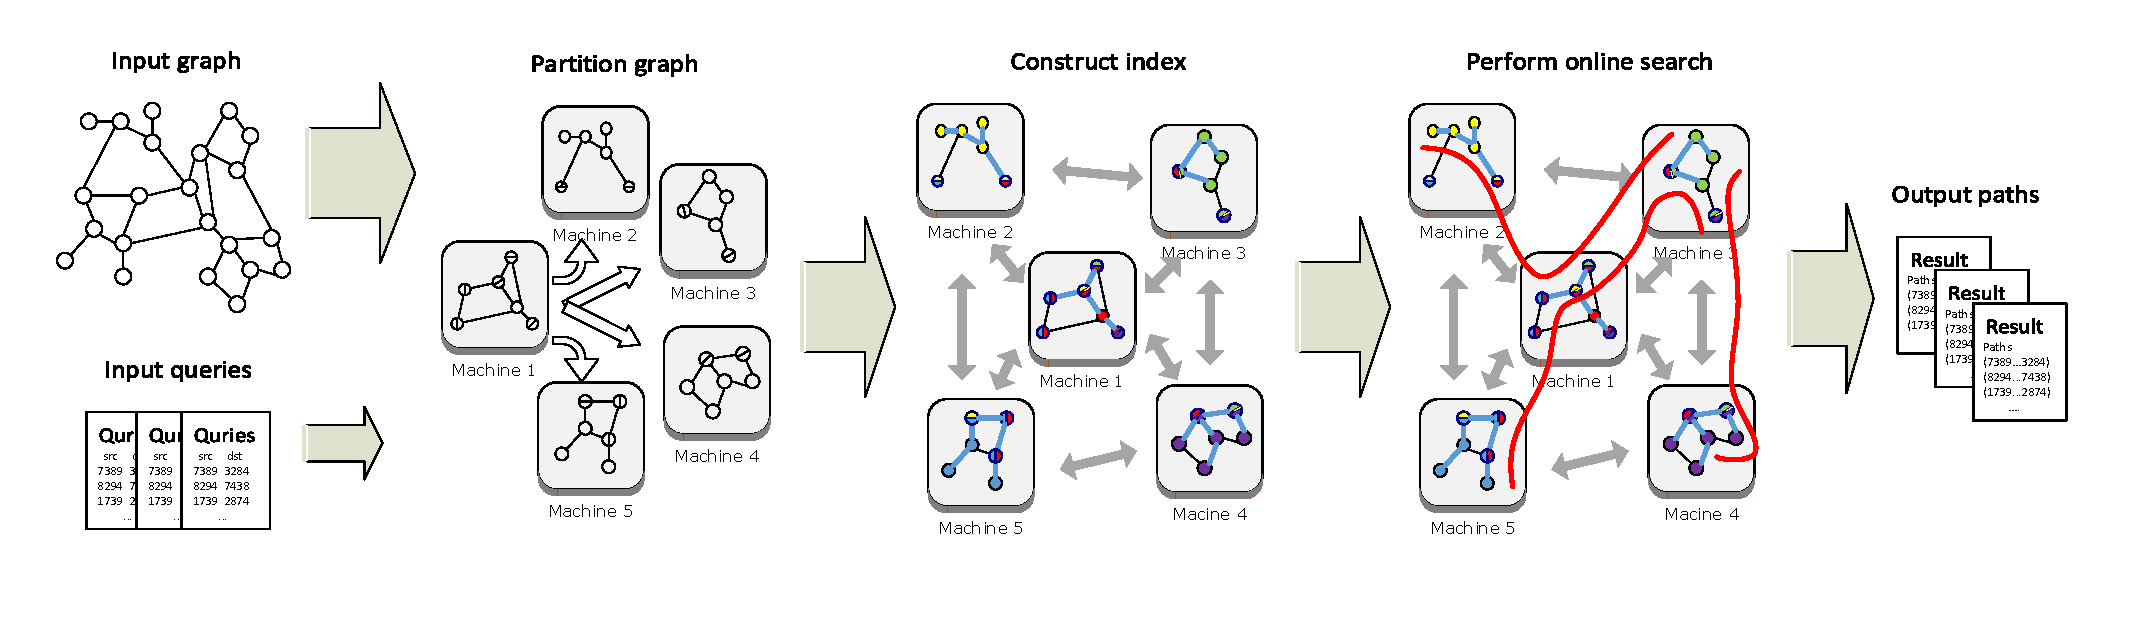
\includegraphics[width=\linewidth]{../figures/new_illustrate/system.pdf}
    \caption{System overview.}
    \label{fig:system}
\end{figure*}

We build our algorithm on a distributed general graph processing platform - Powergraph\cite{180251}. An overview of our system is shown in Fig. \ref{fig:system}. Powergraph is designed to handle large-scale graphs with power law degree distributions efficiently by taking advantage of vertex-programs to factor computation over edges. Computation in Powergraph consists of a vertex-program running on a set of vertices. Each vertex-program consist of three phases: Gather, Apply and Scatter. During Gather phase, the $gather$ and $sum$ functions are used to collect and accumulate data from neighbors. The vertex data is updated in Apply phase by $apply$ function through analysis on data collected from Gather phase. In the Scatter phase, $scatter$ function is used to spread the new value to the graph and signal neighbors to start new vertex-programs. In this section, we are going to talk about details on how we implement our algorithm as vertex-programs.

\subsection{Decentralized search vertex-program}

Algorithm \ref{alg:vc_dec} shows the vertex-program of decentralized search. In Gather phase, for each query, LCA distance $d_L$ calculated from labels $L$ of each neighbor and target vertex is collected and accumulated by finding the neighbor with the smallest LCA distance. If a tie happens, according to our tie strategy, multiple neighbors may be returned as candidates. Since the decentralized search is a state-less search itself, vertex data does not need to be updated during the Apply phase. Instead, the program will append the candidate(s) to the approximated path $p_{appr.}$ and check whether the stop criterion is satisfied for each query. If so, the results will be recorded and this query will be terminated. Otherwise, program will proceed to Scatter phase to start new vertex-programs on next hop candidate(s) of each query and pass query information to them.

\begin{algorithm}
    \caption{Algorithm decentralized search vertex program running on $u$}
		\label{alg:vc_dec}
    \begin{algorithmic}
        \Function{gather}{$L(v)$, $L(t)$}
        %\Comment {Collect LCA distances from Nbrs}
        \State \Return $d_L(v, t)$
        \EndFunction

        \Function{sum}{$d_L(v_1,t)$, $d_L(v_2,t)$}
        %\Comment {Find Nbr with smallest LCA distance to target}
        \State \Return $min(d_L(v_1,t), d_L(v_2,t)$
        \EndFunction

        \Function{apply}{$p_{appr.}(s,t)$, $d_L(v,t)$}
        %\Comment {Update approximate path and check termination}
        \State $p_{appr.}(s,t) += u$
        \If {termination condition meets}
            \State store $p_{appr.}(s,t)$
            \State $term$ = true
        \Else
            \State $term$ = false
        \EndIf
        \EndFunction

        \Function{scatter}{$p_{appr.}(s,t)$, $term$}
        %\Comment {Signal candidates}
        \If {$\neg term$}
            \State Activate(v, $p_{appr.}(s,t)$)
        \EndIf
        \EndFunction
    \end{algorithmic}
\end{algorithm}

\subsection{Index construction vertex-program}
Algorithm \ref{alg:vc_bfs} illustrates the detailed algorithm to perform the BFS to construct the index. Different from regular BFS, when a vertex is visited by a new parent vertex, the path degree $PD$ of the new path and the indexed path will be compared. The label will be updated if the new path has a higher path degree.

Our heuristic index construction vertex-program does not use the gather function. Instead, parent vertices send out messages containing required variables while activating child vertices. Multiple message from different parent vertices will be combined using a message combiner. The rule used here is to compare the value of path degree in order to select the one with the highest path degree.

\begin{algorithm}
    \caption{Algorithm heuristic index construction vertex program running on $u$}
		\label{alg:vc_bfs}
    \begin{algorithmic}
				\Function{msg\_combiner}{$L(v_1)$, $L(v_2)$, $PD(v_1)$, $PD(v_2)$}
				%\Comment {Find Nbr highest path degree}
				\If {$PD(v_1) > PD(v_2)$}
						\State \Return $L(v_1)$, $PD(v_1)$
				\Else
						\State \Return $L(v_2)$, $PD(v_2)$
				\EndIf
        \EndFunction

        \Function{apply}{$L(v)$, $PD(v)$}
        %\Comment {Update label and calculate related path degree}
        \State $L(u) = L(v)$
				\State $L(u).push_back(u.id)$
        \State $PD(u) = PD(v) + u.degree$
        \EndFunction

        \Function{scatter}{$L(u)$, $PD(u)$}
        %\Comment {Signal child vertices}
        \If {$L(v).empty()$}
            \State Activate($v$, $L(u)$, $PD(u)$)
        \EndIf
        \EndFunction
    \end{algorithmic}
\end{algorithm}

\subsection{Breaking ties}

In the centralized version of our search algorithm, ties can be handled very easily. If a candidate cannot lead to the shortest approximate path at the next step among all candidates, it will be simply discarded. The situation becomes more complicated when implementing decentralized search in a distributed setting. In the distributed version of decentralized search, each candidate will start a new vertex program to approximate shortest path independently. There are no communications among different searches as this would be too costly to implement in a distributed setting. Hence, a candidate does not know the length of the path found by other candidates. Even if a candidate finds a shorter path, it does not have the ability to terminate searches at other candidates.

With this limitation, the search space are quite difficult to control and the search may end up with excessive overhead. A naive to alleviate this problem is to set a hard limit on the number of neighbors selected as candidates for next hop. But the algorithm needs to first decide which ones to select, and there is no available information to help making this decision. Another approach used in our implementation is that at each step, only one candidate will be chosen as a ``main'' candidate. For candidates that are not ``main'' candidates, an extra stop criterion will be applied. If it cannot find a shorter path than the one currently found, then the search will stop, and no result will be recorded. This will certainly reduce the chance a shorter path to be found. But it has a much smaller overhead and treats candidates more adaptively than the hard limit approach.

\subsection{Hot-spot prevention}

Our implementation allows millions of decentralized search to run in parallel. But a hot spot problem may arise when running huge number of queries simultaneously. Since paths have more chance to pass a more $central$ vertex, i.e. with a high degree or a high betweenness centrality. When multiple queries running in parallel, a large number of queries will be routed to these $central$ vertices. However, those edges adjacent to these vertices are not necessarily evenly distributed to all machines. So computations may congested on several machines which will lead to larger online search overheads. The power law degree distribution of complex network will intensify this problem. Because it has a very small number of vertices with an extremely high degree. 

The early termination plays an important role in alleviating the hot-spot problems. As the search will not examine any vertices in the labels of target vertex, the least common ancestor will never be traversed. Due to the way decentralized search approximate shortest paths, the least common ancestor is actually the vertex on lowest level of the shortest path tree rooted at the landmark. Note that landmarks are usually high degree vertices in the center part of the graph. And complex networks have a core-fringe structure \cite{callaway2000network}. Vertices on the lower level of the shortest path tree are more likely to have higher degree. So the least common ancestor are likely the highest degree vertex along the approximated path. By avoiding traverse the least common ancestor, the hot-spot problem can be greatly reduced.